%!TEX root = ./intern_report.tex

\newpage
\subsection{The Teal Architecture and Wave Flow Graph(WFG)}
\paragraph{}
Teal is essentially the best of both programmable logic platforms and Application Specific Integrated Circuits(ASIC) combines together to give out the best performance and power efficiencies. In fact both hardware and software designs can be transferred onto the Teal fabric. Basically, Teal can be broken down into smallest unit of a Processing Element(PE). This is a simple processing unit which can carry out 8 bit operations adhering to Reduced Instruction SET (RISC) architecture.

\subsubsection{DPU Architecture}
\paragraph{}
A Processing Element will inherit an 8 bit accumulator who in return is connected to its neighboring Processing Elements. It is evident that a combination of a large number of such Processing Elements achieve as much parallelism as witnessed in the computational design history of the world. This revolutionary design with extensively parallel computational ability is a completely ground-breaking approach to the existing technologies used in chips for parallelism. Incidentally, a combination of 16 Processing Elements make up for a Cluster and a combination of 64 Clusters form a Super-Cluster and 16 such Super-Clusters form a single Wave Dataflow Processing Unit. The projected design for this massively complex structure has now reached the taping out process an it will only be a matter of time before the first chip gets manufactured physically. Such a developed Processing Element is projected to have a speed of close to 10GHz.

\begin{figure}[h]
    \centering
    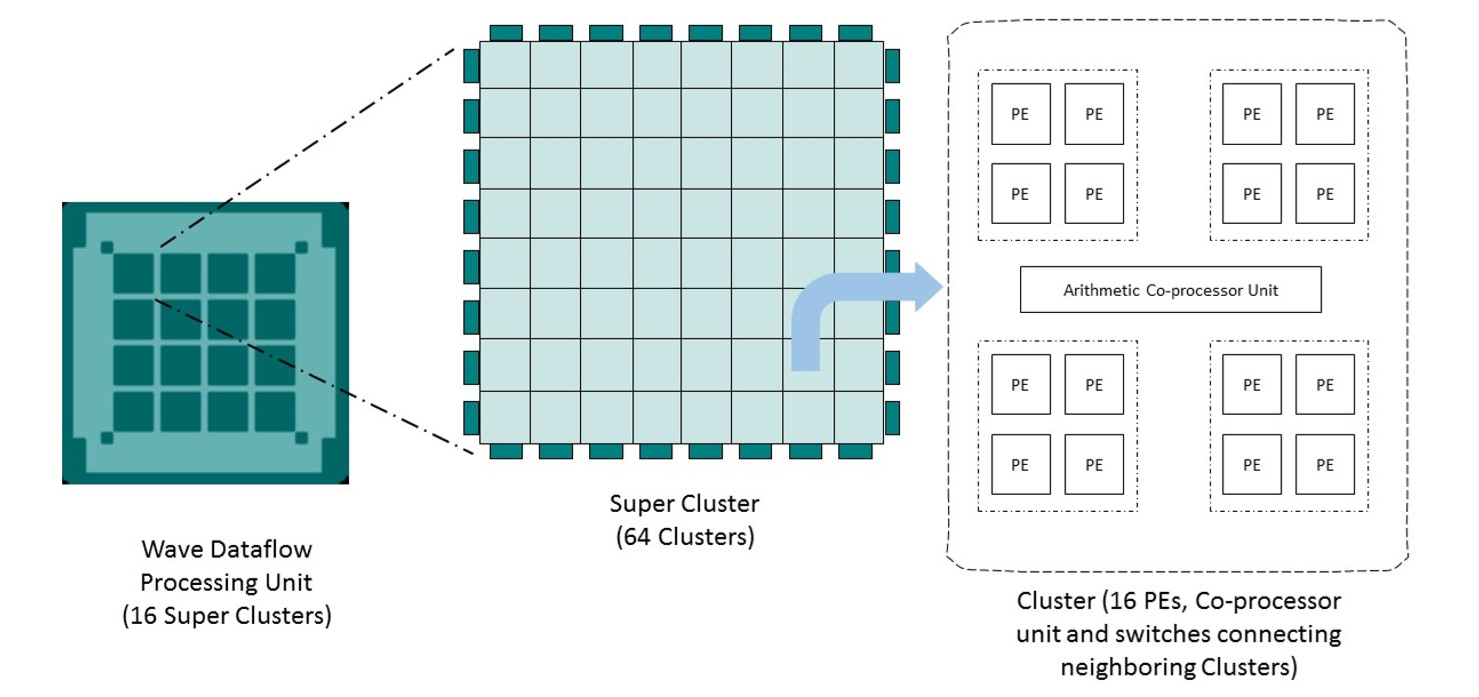
\includegraphics[trim=0cm 0cm 0cm 0cm, clip=true,scale=0.5]{figures/dpu_struct.jpg}
    \caption{Wave DPU with Processing Elements(PEs)\label{Fig:dpustruct}}\vspace{-4mm}
    \end{figure}

\paragraph{}
The Figure~\ref{Fig:dpustruct} is a comprehensive illustration of the structure of Teal design. It is noteworthy to realize that each Processing Element acts much similar to a single processing unit and therefore, each Super Cluster can be viewed in the perspective of thousands of processing units ready to function simultaneously. Nevertheless, the true power of Wave Dataflow Processing Unit design is shown in Figure~\ref{Fig:dpuboard} where the extent of operation of the final design is depicted. The final design is projected to have a whopping 2 Peta Operations per second amount of power which is ideally suited for the needs of computational power of the future. It is safe to say that Wave Dataflow Processing Unit will become by far the fastest ever processing unit of the world.

\begin{figure}[h]
    \centering
    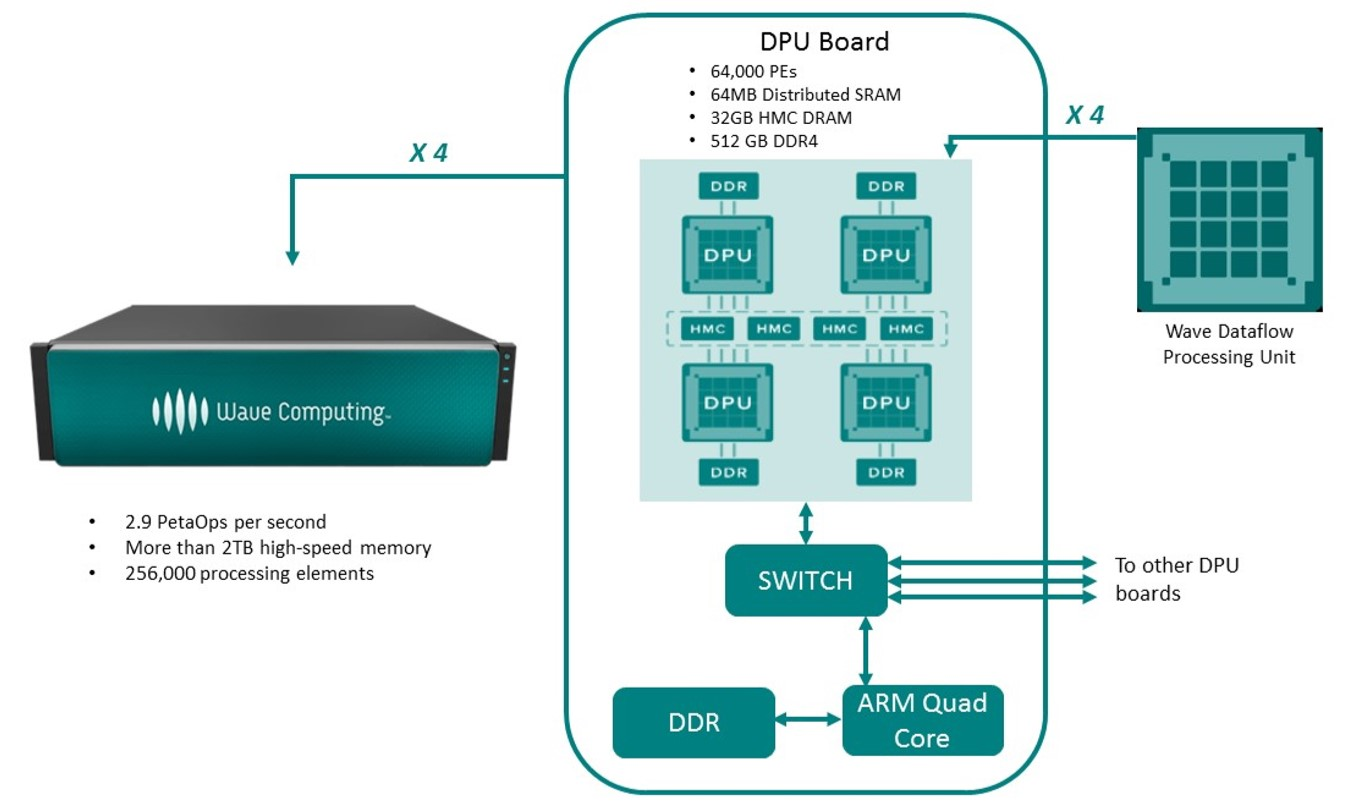
\includegraphics[trim=0cm 0cm 0cm 0cm, clip=true,scale=0.5]{figures/dpu_board.jpg}
    \caption{Wave Deep Learning\label{Fig:dpuboard}}\vspace{-4mm}
    \end{figure}

\subsubsection{SoC Perspective}
\paragraph{}
The Teal processing accelerator is essentially integrated into a System-on-a-Chip(SoC). As shown in the Figure~\ref{Fig:socpers} it is connected to processor SoC using streaming AXI interfaces. It has a direct connection toward high speed IO streams. The DMA controller (refer Figure~\ref{Fig:socpers}) is the key connector between external DRAM internal Block RAMs of Teal. The accelerator itself is demand driven, meaning it will stay at sleep state unless instructed otherwise. The importance of this viewpoint was important to me as some of the design work carried out were finding a way to simulate DMA inputs and outputs. Since accessing data from external RAMs is through DMA ’Channels’, some of the work related to improvements in the DMA engine were carried out during my project executions. 

\paragraph{}
The next interesting design feature of Wave Data-flow processing model are the Wave Flow Graphs. This is a representation scheme for which operations are represented as nodes and values as edges. Nodes and edges connect together in a network of operations to perform a computational task. The idea behind the clock-less operation of the tasks come through the ability for nodes to perform the intended operation whenever valid inputs are provided. A dedicated clock is not needed and thus presence of valid data at the inputs automatically will define trusted operation. 

\paragraph{}
However, a sense of timing is available in the form of the concepts of tics and sub-tics. A tic is equivalent to a circular round of operations executed by a Processing Element buffer which is currently defined as 256 instructions. In fact, it is 256 times the instruction cycle time. Due to the fact that instruction cycle time is not specifically designated but rather dependent on the execution of each operations’ processing speed, it is not fair by the Wave DPU design to have a specific tic-rate. Incidentally, there is a typical rate of 10 GHz for a sub-tic cycle. a sub-tic cycle is essentially the rate at which an instruction from a circular buffer(IRAM) is fetched, processed and switched. 

\begin{figure}[h]
    \centering
    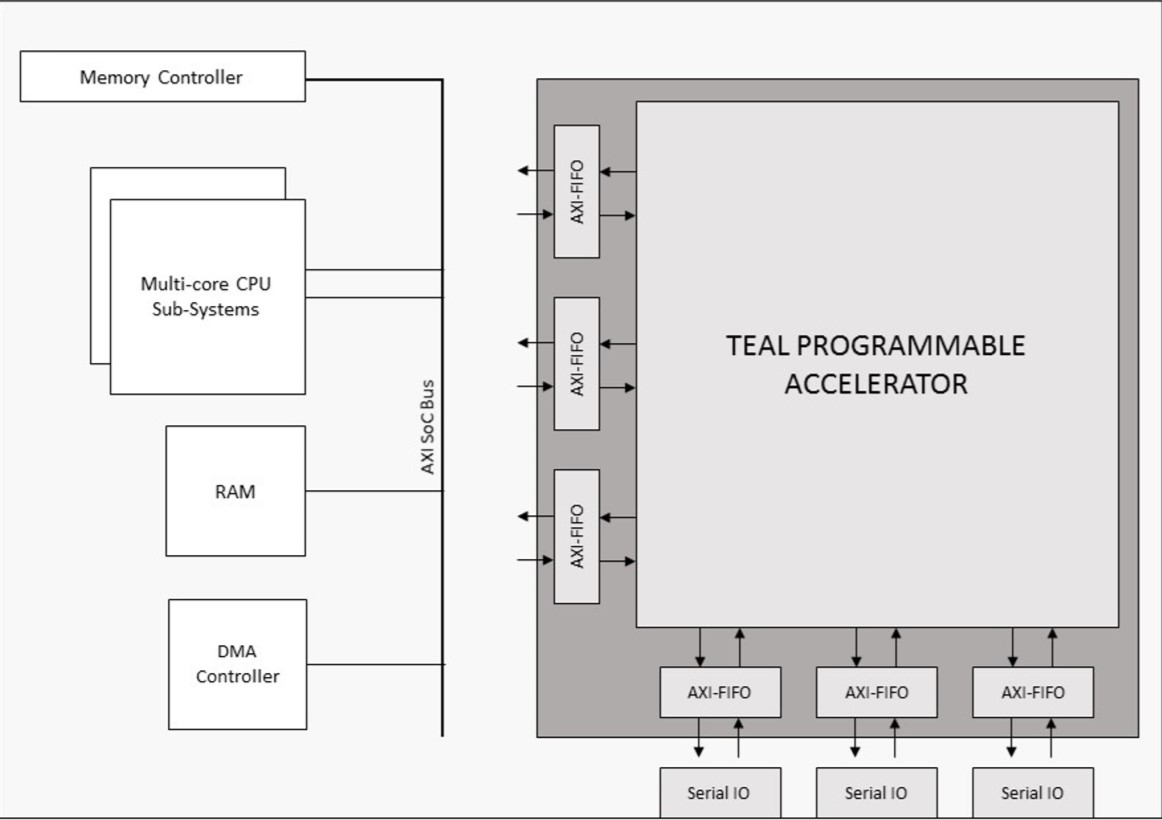
\includegraphics[trim=0cm 0cm 0cm 0cm, clip=true,scale=0.5]{figures/soc_pers.jpg}
    \caption{SoC Perspective of Teal Programmable Accelerator\label{Fig:socpers}}\vspace{-4mm}
    \end{figure}

\paragraph{}
Apart from the contrast between the parallelized implementation of Wave Flow Graph designs and the continuous flow of operations within PEs, Wave Flow Graph is a defined rule to represent any program within the Teal fabric. In XXXXXXX section 1.3.3 (Unit Testing) XXXXXX a direct implementation of testing the Wave Flow Graph operations carried out by me, is explained in detail.

\subsubsection{Wave design flow}
\paragraph{}
Owing to the complexity of parallel PE operation it is evidently clear that programming instructions into the Teal Architecture is not achievable manually. Therefore, an EDA flow is prevalent so that any hardware design can be brought down through compilation, scheduling, mapping and routing to the Teal fabric level. This flow of compilation from hardware design to Byte-fabric level is done through the Wave introduced design flow. The Figure~\ref{Fig:wfgstruct} is a representation of a very simple Wave Flow Graph design where you can see the nature of operation of the language. It basically consists of bit wise operations between inputs and outputs. Most operations are related to bit level manipulation of data and it is note worthy to realize that these operations are carried out for 8 bit data chunks. The combination of several bytes of data can be processed with special modules of Wave Flow Graph code where the data is subdivided and processed accordingly. The node edge representation of the design will give you enough ides as to the complexity that can arise with the introduction of several operations and variables into one design. The final structure will be a collection of various nets combined together from input end to output end.

\begin{figure}[h]
    \centering
    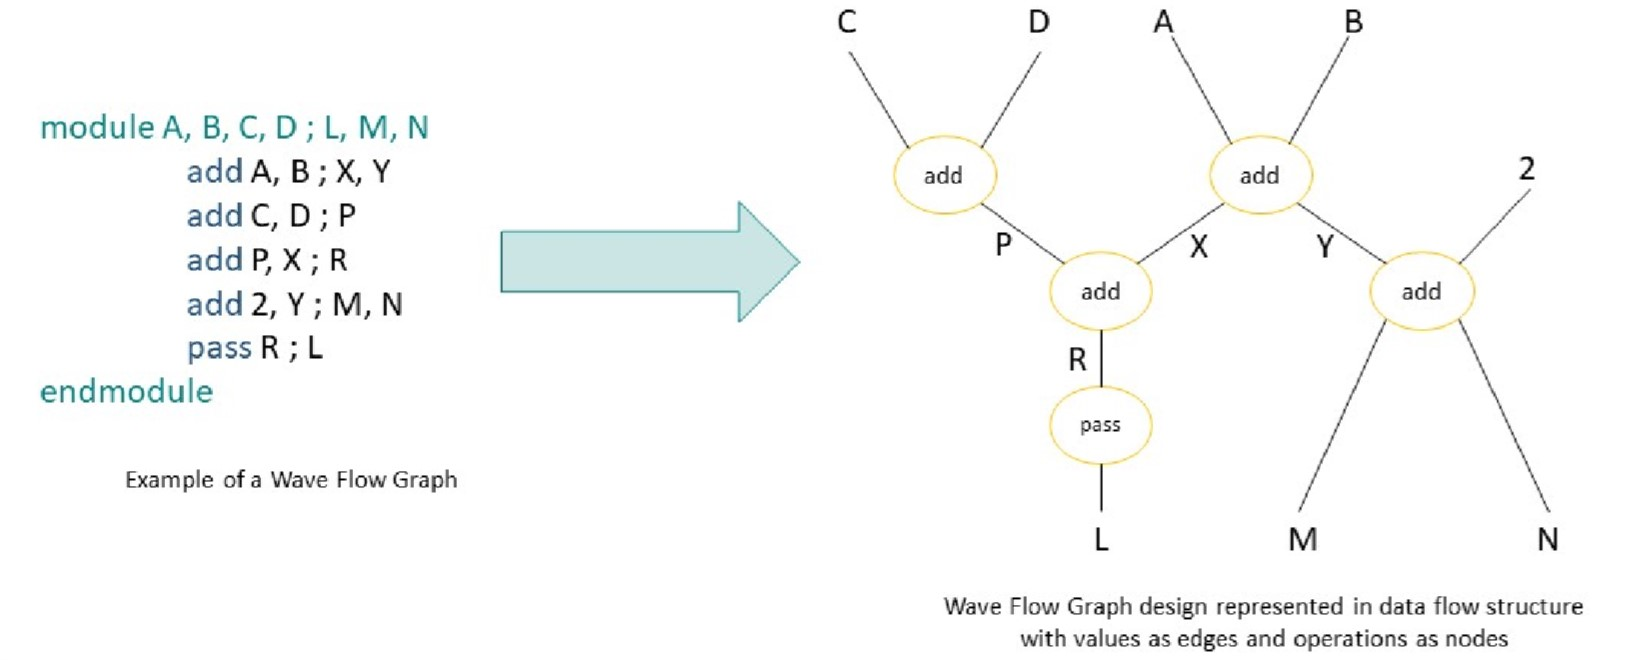
\includegraphics[trim=0cm 0cm 0cm 0cm, clip=true,scale=0.5]{figures/wfg_struct.jpg}
    \caption{Data flow structure of Wave Flow Graph designs\label{Fig:wfgstruct}}\vspace{-4mm}
    \end{figure}